%Please use LuaLaTeX or XeLaTeX
\documentclass[11pt,aspectratio=169]{beamer}

\title{Theta Functions, Kronecker Functions, and Bilinear Relations}
\date[2023]{Riemann Surfaces \\ in Mathematical Physics}
\author{Artyom Lisitsyn}
\institute{D-PHYS}

\usetheme{eth}

\colorlet{titlefgcolor}{ETHBlue}
\colorlet{accentcolor}{ETHRed}

\usepackage{cancel}

\newcommand{\ee}[0]{\mathbf{e}}

\begin{filecontents}{\jobname.bib}
    @book{Ber06,
        Author = {Marco Bertola},
        Title = {Riemann Surfaces and Theta Functions},
        Year = {2006}}

    @thesis{Cha22,
        Author = {Zhi Cong Chan},
        Title = {Towards a Higher-Genus Generalization of the
        Kronecker Function Using Schottky Covers},
        Year = {2022}
    }

    @misc{BL13,
      title={Multiple Elliptic Polylogarithms},
      author={Francis C. S. Brown and Andrey Levin},
      year={2013},
      archivePrefix={arXiv},
      primaryClass={math.NT},
    }
\end{filecontents}
\usepackage[backend=bibtex,style=authoryear, defernumbers=true]{biblatex}
\addbibresource{\jobname.bib}
\begin{document}

% Find better title image?
\def\titlefigure{elements/title-page-image}
\titleframe{}

\tocframe{}

\section{Abel's map}

\begin{frame}{Holomorphic Differentials}
    \begin{block}{Existence of holomorphic differentials}
        The dimension of the space of holomorphic differentials is $\dim \mathcal H^1 = g$, the genus of the compact Riemann surface.
    \end{block}

    \begin{columns}[onlytextwidth]
        \begin{column}{0.55\textwidth}
            \emph{Proof outline:}
            \begin{itemize}
                \item $\dim \mathcal H^1 \leq \text{\# of a-cycles} = g$
                \item $\text{\# of harmonic differentials} = \dim H \geq 2g$
                \item $h = f dz + g d \bar z \implies \dim H = 2 \dim \mathcal H^1$
                \item $g \leq \dim \mathcal H^1 \leq g \implies \dim \mathcal H^1 = g$
            \end{itemize}
            \emph{Normalization \& period matrix:}
            \[ \int_{a_i} \omega_j = \delta_{ij} \]
            \[ \int_{b_i} \omega_j = \tau_{ij} \]
        \end{column}
        \begin{column}{0.45\textwidth}
            \center{}
            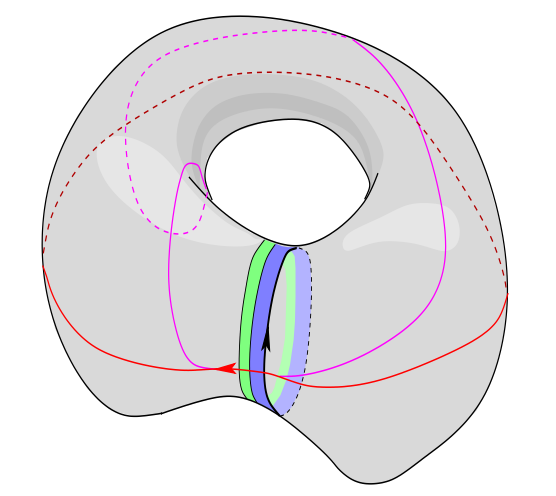
\includegraphics[width=0.8\columnwidth]{assets/HarmonicDifferential.png}
            
            \tiny Regions used to define harmonic differentials

            \cite{Ber06}
        \end{column}
    \end{columns}
\end{frame}

\begin{frame}{Abel's map}{\tiny \cite{Ber06} Section 4.2}
    \begin{columns}
        \begin{column}{0.55\textwidth}
            \begin{block}{Formal definition of Abel's map}
                For a particular choice of a point $P_0$ on the fundamental domain $\mathcal L$, using the normalized harmonic differentials $\omega_i$, we have Abel's map
                \begin{align*}
                    \mathbf{u} : \mathcal L & \mapsto \mathbb{C}^g , \quad P & \mapsto \begin{pmatrix} \int_{P_0}^P \omega_1 \\ \vdots \\ \int_{P_0}^P \omega_g \end{pmatrix} &
                \end{align*}
            \end{block}
        \end{column}
        \begin{column}{0.45\textwidth}
            \center

            \includegraphics[width=0.7\columnwidth]{example-image-a}

            \tiny Fundamental domain

            \cite{ImageSource}
        \end{column}
    \end{columns}

    \emph{Analytic continuation beyond the fundamental domain:}
    \[\mathbf{u}(P+a_i) = \mathbf{u}(P) + \begin{pmatrix} \int_{a_i} \omega_1 \\ \vdots \end{pmatrix} = \mathbf{u}(P) + \begin{pmatrix} \delta_{i1} \\ \vdots \end{pmatrix}\]
    \[\mathbf{u}(P+b_i) = \mathbf{u}(P) + \begin{pmatrix} \tau_{i1} \\ \vdots \end{pmatrix}\]
\end{frame}

\begin{frame}{Abel's map at genus 1}
    \begin{columns}[onlytextwidth]
        \begin{column}{0.55\textwidth}
            Appropriate differential
            \[\omega = dz\]
            
            Abel's map
            \[\mathbf{u}(z) = \int_0^z \omega = z\]
        \end{column}
        \begin{column}{0.45\textwidth}
            \center{}
            \includegraphics[width=0.7\columnwidth]{example-image-a}

            \tiny Fundamental domain and continuation at genus 1

            \cite{ImageSource}
        \end{column}
    \end{columns}

    {
    % \setbeamercolor{block body}
    \setbeamercolor{block title}{bg=ETHBlue}
    \setbeamercolor{block body}{bg=ETHBlue!25!white}
    \begin{block}{What about higher genus?}
        \begin{itemize}
            \item How do we represent the fundamental domain?
            \item What choice of differentials can we make?
            \item What consequences does this have for Abel's map?
        \end{itemize}
    \end{block}
    }
\end{frame}

\section{Theta functions}

\begin{frame}{Theta functions}{\tiny \cite{Ber06} Section 5.1}
    \begin{block}{Definition of the Theta function}
        Given a symmetric matrix $\tau$ with positive definite imaginary part, the Theta function is
        \[\Theta(\vec z, \tau) := \sum_{\vec n \in \mathbb Z^g} \ee \left( \frac{1}{2} \vec n^T \tau \vec n + \vec n^T \vec z \right) \quad , \quad \ee(z) = \exp(2\pi i z)\]
    \end{block}
    % \pause
    \emph{Properties:} For $\vec \lambda \in \mathbb Z^g$

    \[\Theta(-\vec z) \overset{\vec n \mapsto -\vec n}{=} \Theta(\vec z)\]
    % \pause
    \[\Theta(\vec z + \vec \lambda) = \sum_{\vec n \in \mathbb Z^g} \cancelto{1}{\ee ( \vec n^T \vec \lambda)} \ee(\ldots) = \Theta(\vec z)\]
    % \pause
    \[\Theta(\vec z + \tau \vec \lambda) = \begin{bmatrix} \text{shift } \vec n \\ \text{use }\tau\text{ symmetry}\end{bmatrix} = \ee \left(- \frac{1}{2}\vec \lambda^T \tau \lambda-\vec \lambda^T \vec z\right)\Theta(\vec z)\]
\end{frame}

\begin{frame}{Theta function on a compact Riemann surface}{\tiny \cite{Ber06} Section 5.2}
    \begin{block}{Definition of Theta function on a compact Riemann surface}
        For a compact Riemann surface $\mathcal M$ of genus $g$, with period matrix $\tau$ and Abel's map $\mathbf{u}$, we can identify
        \begin{align*}
            \theta : \ & \mathcal M \mapsto \mathbb C \\
            & P \mapsto \Theta(\mathbf{u}(P))
        \end{align*}
    \end{block}

    \emph{Properties:}
    \[ \theta(P + a_i) = \theta(P) \]

    \[ \theta(P + b_i) = \ee\left(- \frac{1}{2} \tau_{ii} - \mathbf{u}_i(P)\right)\theta(P) \]
\end{frame}

\begin{frame}{Theta function at genus 1}
    \begin{columns}[onlytextwidth]
        \begin{column}{0.55\textwidth}
            \[\theta(z) = \sum_{n \in \mathbb Z} \ee(\frac{1}{2}n^2 \tau + n z)\]

            \[\theta(z)=\theta(-z)\]
            \[\theta(z+1)=\theta(z)\]
            \[\theta(z+\tau)=\ee(-\frac{1}{2}\tau-\xi)\theta(z)\]
        \end{column}
        \begin{column}{0.45\textwidth}
            \center{}
            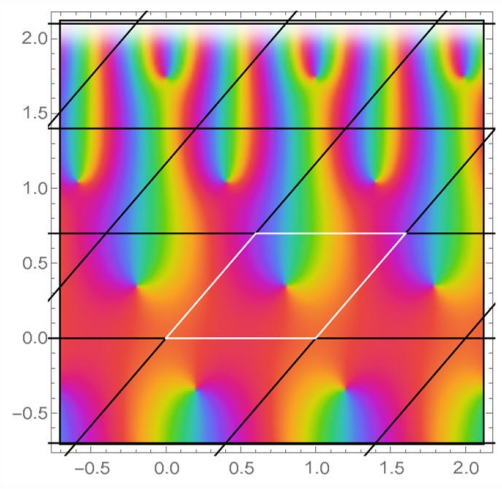
\includegraphics[width=0.7\columnwidth]{assets/genus1theta.png}

            \tiny Theta function for $\tau = 0.7+0.6i$
            
            \cite{Cha22}
        \end{column}
    \end{columns}

    {
    % \setbeamercolor{block body}
    \setbeamercolor{block title}{bg=ETHBlue}
    \setbeamercolor{block body}{bg=ETHBlue!25!white}
    \begin{block}{What about higher genus?}
        \begin{itemize}
            \item What does the Theta function look like at higher genus?
        \end{itemize}
    \end{block}
    }
\end{frame}

\begin{frame}{Theta function with characteristics}{\tiny \cite{Ber06} Section 5.1}
    \begin{block}{Definition of Theta function with characteristics}
        Consider vectors $ \epsilon ,  \epsilon' \in \mathbb R^g$.
        We can then define the Theta function with characteristics $ \epsilon$, $ \epsilon'$ as
        \[\Theta\begin{bmatrix} \epsilon \\  \epsilon'\end{bmatrix}(\vec z) := 
        \ee\left(\frac{1}{8}\epsilon^T \tau \epsilon + \frac{1}{2}\epsilon^T \vec z + \frac{1}{4}\epsilon^T  \epsilon'\right)
        \Theta(\vec z + \frac{\epsilon'}{2}+\frac{\tau\epsilon}{2})\]
    \end{block}
    % \pause
    \emph{Properties:}

    \[\Theta\begin{bmatrix}\epsilon \\ \epsilon'\end{bmatrix}(\vec z + \vec \alpha + \tau \vec \beta) =
    \ee\left(\frac{1}{2}(\epsilon^T \vec \alpha - \vec \beta^T \epsilon') - \frac{1}{2} \beta^T \tau \beta - \vec \beta \vec z\right)
    \Theta\begin{bmatrix}\epsilon \\ \epsilon'\end{bmatrix}(\vec z)\]
    % \pause
    \[\Theta\begin{bmatrix}\epsilon + 2\eta \\ \epsilon' + 2\eta' \end{bmatrix}(\vec z) = \exp(\pi i \epsilon^T \eta')
    \Theta\begin{bmatrix}\epsilon \\ \epsilon'\end{bmatrix}(\vec z) \quad , \quad \eta,\eta' \in \mathbb Z^g\]
    % \pause
    \[\Theta\begin{bmatrix}\epsilon \\ \epsilon'\end{bmatrix}(-\vec z) = \exp(\pi i \epsilon^T \epsilon') \Theta\begin{bmatrix}\epsilon \\ \epsilon'\end{bmatrix}(\vec z) \quad , \quad \epsilon,\epsilon' \in \mathbb Z^g\]
\end{frame}

\begin{frame}{Odd theta functions and zeros}
    \begin{columns}[onlytextwidth]
        \begin{column}{0.55\textwidth}
            \begin{align*}
                & \epsilon,\epsilon' \in \mathbb Z^g , \quad \epsilon^T \epsilon'\text{ is odd} \\
                & \Theta\begin{bmatrix}\epsilon \\ \epsilon'\end{bmatrix}(-\vec z) = \exp(\pi i \epsilon^T \epsilon') \Theta\begin{bmatrix}\epsilon \\ \epsilon'\end{bmatrix}(\vec z)
                \\
                & \implies \Theta\begin{bmatrix}\epsilon \\ \epsilon'\end{bmatrix}(\vec z) = \Theta\begin{bmatrix}\epsilon \\ \epsilon'\end{bmatrix}(-\vec z)
                \\
                & \implies \Theta\begin{bmatrix}\epsilon \\ \epsilon'\end{bmatrix}(0) = \Theta\begin{bmatrix}\epsilon \\ \epsilon'\end{bmatrix}(\vec \lambda' + \tau \vec \lambda) = 0
                \\
                & \implies \Theta(\frac{\epsilon'}{2}+\frac{\tau\epsilon}{2}) = 0
            \end{align*}
        \end{column}
        \begin{column}{0.45\textwidth}
            \center{}
            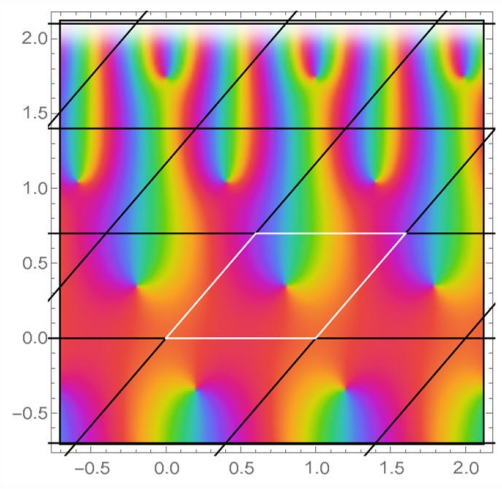
\includegraphics[width=0.7\columnwidth]{assets/genus1theta.png}

            \tiny Theta function for $\tau = 0.7+0.6i$
            
            \cite{Cha22}
        \end{column}
    \end{columns}

    {
        % \setbeamercolor{block body}
        \setbeamercolor{block title}{bg=ETHBlue}
        \setbeamercolor{block body}{bg=ETHBlue!25!white}
        \begin{block}{What about higher genus?}
            \begin{itemize}
                \item Which of the zeros located by odd characteristics are actually reached by Abel's map on compact Riemann surfaces of higher genus?
            \end{itemize}
        \end{block}
    }
\end{frame}

\begin{frame}{Odd theta function at genus 1}
    \begin{block}{Odd theta function at genus 1}
        We define
        \[\theta_1(z) = -\theta \begin{bmatrix} 1 \\ 1 \end{bmatrix}(z)\]
        It has equivalent definition
        \[\theta_1(z) = 2iq^{1/8} \sin(\pi z) \prod_j (1-q^j) (1-wq^j)(1-w^{-1}q^j) \quad , \quad q=\ee(\tau)\]
    \end{block}
    \emph{Jacobi Triple Product:}
    % https://en.wikipedia.org/wiki/Jacobi_triple_product
    % https://en.wikipedia.org/wiki/Theta_function
    \[f(x,y) = \prod_{j>0} (1-x^{2m})(1+x^{2m-1}y^2)(1+x^{2m-1}y^{-2})\]
    \[f(x,xy) = \prod_{j>0} (1-x^{2m})(1+x^{2m+1}y^2)(1+x^{2m-3}y^{-2}) = \frac{1+x^{-1}y^{-2}}{(1+xy^2)}f(x,y) = x^{-1}y^{-2}f(x,y)\]
\end{frame}

\begin{frame}{Odd theta function at genus 1}
    \[f(x,y) = \prod_{j>0} (1-x^{2m})(1+x^{2m-1}y^2)(1+x^{2m-1}y^{-2})\]
    \[f(x,xy) = \prod_{j>0} (1-x^{2m})(1+x^{2m+1}y^2)(1+x^{2m-3}y^{-2}) = \frac{1+x^{-1}y^{-2}}{(1+xy^2)}f(x,y) = x^{-1}y^{-2}f(x,y)\]
    % \pause
    \[f(x,y) = \sum_{n=-\infty}^\infty c_n(x) y^{2n} \implies f(x,y) = xy^2 f(x,xy) = \sum_n c_n(x) x^{2n+1}y^{2n+2}\]
    \[\implies c_{n+1}(x) = x^{2n+1}c_n(x) \implies c_{n}(x) = c_0(x) x^{n^2} \implies f(x,y) = c_0(x) \sum_n x^{n^2} y^{2n}\]

    This relates the two forms of the theta function : $\prod_j (1-q^j) (1-wq^j)(1-w^{-1}q^j) \simeq \sum_n \ee(\tau)^{n^2} \ee{z}^{n}$

    {
        % \setbeamercolor{block body}
        \setbeamercolor{block title}{bg=ETHBlue}
        \setbeamercolor{block body}{bg=ETHBlue!25!white}
        \begin{block}{What about higher genus?}
            \begin{itemize}
                \item Are there similar formulas for higher genus theta functions that make them easier to work with in some cases?
            \end{itemize}
        \end{block}
    }
\end{frame}

\begin{frame}{(Application) Decomposing meromorphic functions}{\tiny \cite{Cha22} Section 3.4 \& \cite{Ber06} Chapter 6}
    Rough outline of how to reproduce a function with divisor $(f) = \sum n_i P_i$
    \[ \begin{bmatrix}\text{Find function }t(z) \\ \text{such that }t(0)=0\end{bmatrix} \rightarrow \begin{bmatrix} g(z)=\prod t(P-P_i)^{n_i} \\ \text{respecting possible periodicity}\end{bmatrix} \rightarrow \left(\frac{f}{g}\right) = \emptyset \rightarrow \frac{f}{g} = \text{const.} \]
    Recall that $\deg((f)) = \sum n_i = 0$ for meromorphic functions.
    % \pause
    \vspace{+1em}
    \begin{columns}[t]
        \begin{column}{0.3\textwidth}
            Genus 0:
            \begin{itemize}
                \item $f(z) = C \prod (z-z_i)^{n_i}$
            \end{itemize}
        \end{column}

        \begin{column}{0.3\textwidth}
            Genus $>0$:
            \begin{itemize}
                \item $\Theta(\xi) = 0$
                \item $g_{P'} : P \mapsto \Theta(\mathbf{u}(P)-\mathbf{u}(P')+\xi)$
                \item $f(P) = C \prod \left(g_{P_i}(P)\right)^{n_i}$
            \end{itemize}
        \end{column}

        \begin{column}{0.35\textwidth}
            Genus 1:
            \begin{itemize}
                \item Decompose $z_i = \frac{b_i}{2} + \tau \frac{a_i}{2}$
                \item $f(z) = C \prod \left(\theta\begin{bmatrix}a_i \\ b_i\end{bmatrix}(z)\right)^{n_i}$
            \end{itemize}
        \end{column}
    \end{columns}
\end{frame}

\section{Kronecker function}

\begin{frame}{Kronecker function}{\tiny \cite{BL13} Section 3.4}
    \begin{block}{Definitions of the Kronecker function}
        The Kronecker function $F(\xi,\eta,\tau)$ has equivalent definitions
        \begin{enumerate}
            \item In terms of the odd theta function
            \[\frac{\theta_1'(0)\theta_1(\xi+\eta)}{\theta_1(\xi)\theta_1(\eta)}\]
            \item In terms of a sum over exponentials
            \[-2\pi i \left(\frac{z}{1-z} + \frac{1}{1-w} + \sum_{m,n > 0} (z^m w^n - z^{-m} w^{-n}) q^{mn}\right) \quad , \quad \begin{pmatrix} z \\ w \\ q \end{pmatrix} = \ee \begin{pmatrix}\xi \\ \eta \\ \tau\end{pmatrix}\]
            \item In terms of a sum over Eisenstein functions and series
            \[\frac{1}{\eta} \exp\left(-\sum_{j > 0} \frac{(-\eta)^j}{j} (E_j(\xi,\tau) - e_j(\tau))\right)\]
        \end{enumerate}
    \end{block}
\end{frame}

\begin{frame}{Properties of the Kronecker function}{\tiny \cite{BL13} Section 3.4}
    \emph{Properties:}
    \[F(\xi+1,\eta) = \frac{\theta_1'(0)\theta_1(\xi+\eta+1)}{\theta_1(\xi+1)\theta_1(\eta)} = F(\xi,\eta)\]
    % \pause
    \[F(\xi+\tau,\eta) = \frac{\theta_1'(0)\theta_1(\xi+\eta+\tau)}{\theta_1(\xi+\tau)\theta_1(\eta)} = \frac{\ee(-\xi-\eta)}{\ee(-\xi)} F(\xi,\eta)\]
    % \pause
    \[FAY RELATION\]
\end{frame}

\begin{frame}{Abridged derivation of the Fay relation}

\end{frame}

\begin{frame}{Differentials from the Kronecker function}
    showing how the expansion is done
\end{frame}

\begin{frame}{Examples of differentials}
    [1412.5535] eqn 3.31 etc.
\end{frame}

\begin{frame}{Independence of the differentials}
    Brown and Levin
    (probably needs to be several slides)
\end{frame}

\begin{frame}{Fay relation for differentials}
    one line derivation
    one line statement
\end{frame}

\begin{frame}{Application of properties}
    big picture view of when these come into string theory
\end{frame}

\section{Striving for higher genus}

\begin{frame}{Why we care about higher genus}
    Connection to string theory
\end{frame}

\begin{frame}{Questions gathered so far}
    {
        % \setbeamercolor{block body}
        \setbeamercolor{block title}{bg=ETHBlue}
        \setbeamercolor{block body}{bg=ETHBlue!25!white}
        \begin{block}{What about higher genus?}
            \begin{itemize}
                \item How do we represent the fundamental domain?
                \item What choice of differentials can we make?
                \item What consequences does this have for Abel's map?
                \item What does the Theta function look like at higher genus?
                \item Which of the zeros located by odd characteristics are actually reached by Abel's map on compact Riemann surfaces of higher genus?
            \end{itemize}
        \end{block}
    }
\end{frame}

\begin{frame}{Schottky cover definition}

\end{frame}

\begin{frame}{Schottky group example}

\end{frame}

\begin{frame}{Differentials and theta functions}

\end{frame}

\begin{frame}{Attempt at a Kronecker function}{\tiny \cite{Cha22}}

\end{frame}

\begin{frame}{Open questions}

\end{frame}

\begin{frame}{References}
    \printbibliography{}
\end{frame}

\end{document}